\documentclass[aspectratio=169,11pt]{beamer}

\usetheme{Boadilla}
\usecolortheme{seahorse}
\useinnertheme{rounded}
\useoutertheme{infolines}

\usepackage{booktabs}
\usepackage{graphicx}
\usepackage{xcolor}
\usepackage{tikz}

% Figürler iki yerden çekilebilsin
\graphicspath{{../phase-2/}{../phase-3/}}

% Tek tip görünüm için renkler
\definecolor{accent}{HTML}{1f4e79}
\definecolor{warn}{HTML}{c0392b}
\definecolor{ok}{HTML}{27ae60}

\setbeamercolor{title}{fg=accent}
\setbeamercolor{frametitle}{fg=accent}
\setbeamercolor{structure}{fg=accent}

% Sayfa numarası gizle alt bar'da minimal
\setbeamertemplate{navigation symbols}{}

% ---------------- META ----------------
\title[When Does Text Help?]{When Does Text Help?}
\subtitle{A Leakage-Free Information-Richness and\\
Encoder-Adaptation Study for Multimodal\\
Land-Cover Composition Regression}
\author[Ö.\,F.~Merey]{Ömer Faruk Merey}
\institute[METU]{Graduate School of Informatics\\Middle East Technical University}
\date{DI 725 --- Final Presentation}

\begin{document}

% ---------- 1. TITLE ----------
\begin{frame}
  \titlepage
\end{frame}

% ---------- 2. PROBLEM ----------
\begin{frame}{Problem}
\begin{columns}[T]
  \column{0.58\textwidth}
  \large
  Predict the \textbf{land-cover composition}\\of a satellite tile:
  \medskip
  \begin{itemize}\setlength\itemsep{2pt}\normalsize
    \item 7 mutually exclusive classes\\
          (Tree, Shrub, Grass, Crop, Built-up, Barren, Water)
    \item Percentages sum to 100\,\%
    \item \textbf{Regression}, not classification
  \end{itemize}
  \medskip
  \normalsize
  \textbf{Hypothesis:} text captions describing the tile could help a vision model.
  \medskip
  \textbf{Question:} \emph{Does adding text actually help --- and can we measure it honestly?}
  \column{0.42\textwidth}
  \centering
  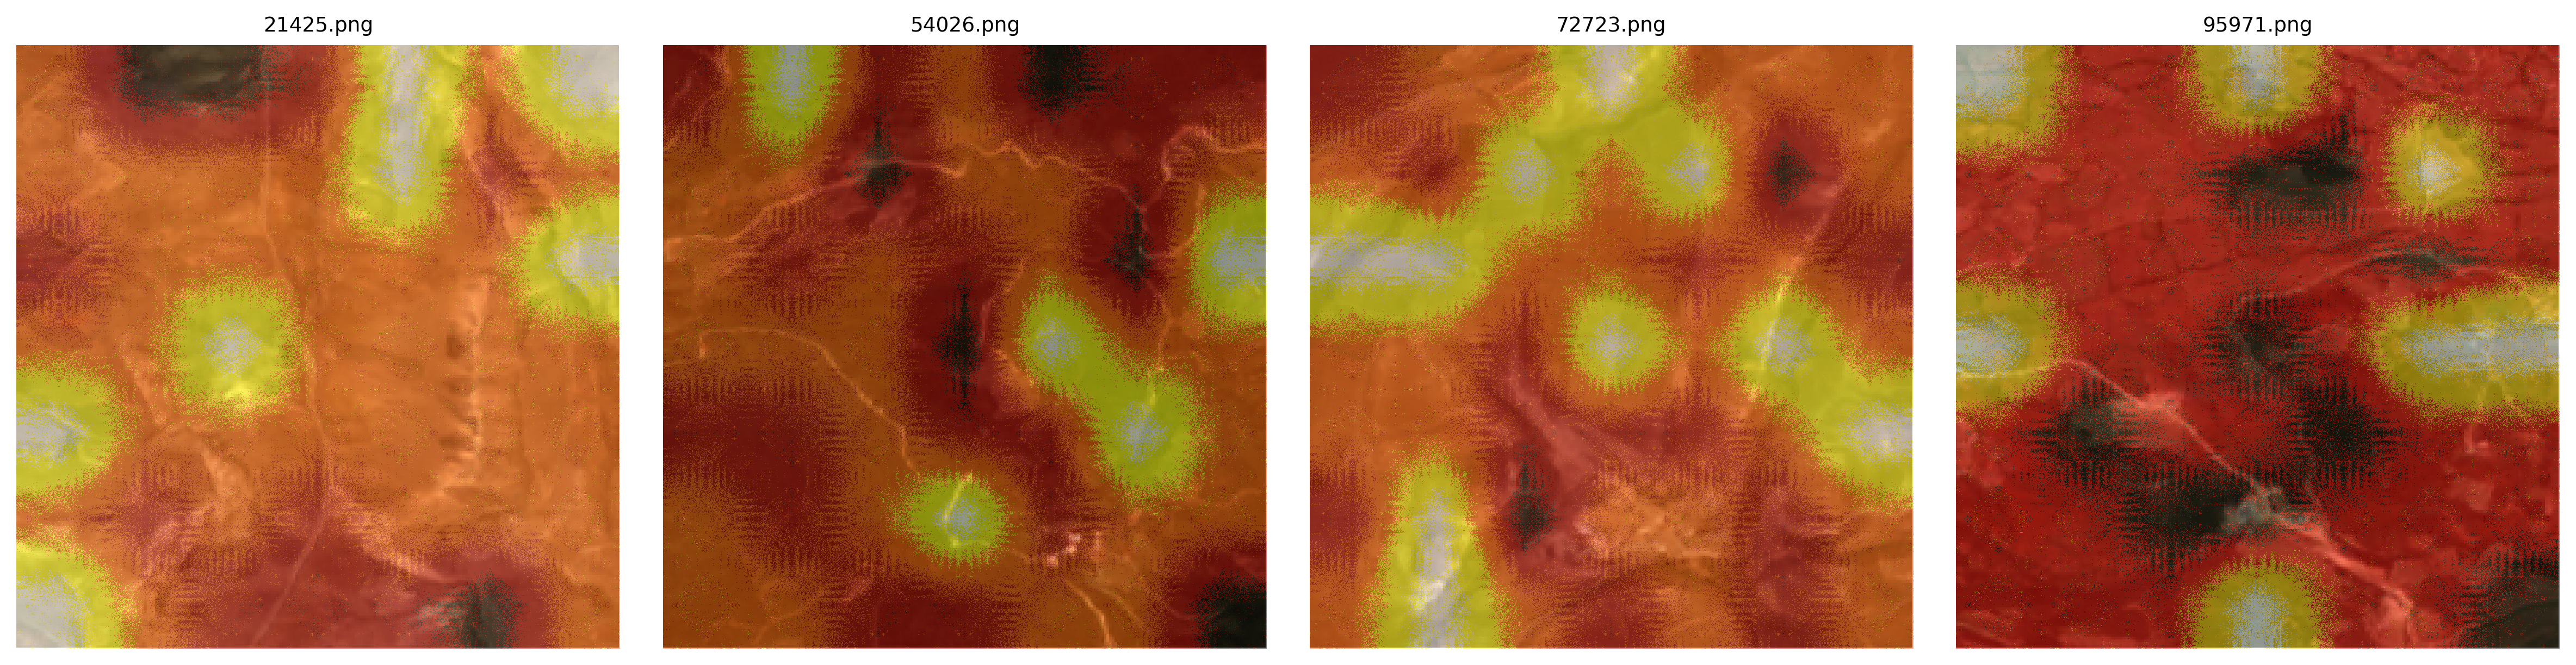
\includegraphics[width=\linewidth]{phase2_attention.png}\\
  {\scriptsize Cross-attention overlays on ARAS400k tiles}
\end{columns}
\end{frame}

% ---------- 3. DATASET + PHASE 1 ----------
\begin{frame}{Dataset \& Phase 1 (PoC)}
\textbf{ARAS400k}: 10\,000 RGB tiles ($256{\times}256$), pixel masks, \textbf{5 caption variants}.
\medskip

\textbf{Architecture (proof-of-concept):}
\smallskip

\begin{center}
\small
$\underbrace{\text{Image}}_{\text{CLIP ViT-B/32}}
\!\to\! \underbrace{49\text{ patch tokens}}_{Q}\;
+\;\underbrace{77\text{ text tokens}}_{K,\,V}$\\[3pt]
$\to\;\text{8-head cross-attention}\;\to\;\text{mean-pool}\;\to\;\text{MLP}\;\to\;\text{7\,\% (softmax)}$
\end{center}
\smallskip

\textbf{Loss:} MSE on softmax output vs.\ GT/100.\\[6pt]

Phase~1 was a \emph{single-sample forward pass} --- pipeline validation only, no training yet.
\end{frame}

% ---------- 4. THE TWIST ----------
\begin{frame}{\textcolor{warn}{The Twist}: Data Leakage}
\begin{block}{3 of 5 caption variants embed GT \% \textbf{verbatim}}
\small
\begin{tabular}{@{}ll@{}}
\texttt{hybrid\_gemma3-4b}    & \emph{``grasslands (92\%) with sparse barren land (6\%)''} \\
\texttt{hybrid\_qwen3-vl-8b}  & \emph{``grassland covering 92\% of the area''} \\
\texttt{text\_qwen3-4b}       & \emph{``predominantly covered by grass\dots''} \\
\end{tabular}
\end{block}

\medskip
A model trained on these solves the task \textbf{lexically} --- it reads the answer.

\medskip
\textbf{Crucially:} stripping digits is not enough. The VLMs that wrote those captions
\emph{saw} the GT, so even qualitative narrative carries label structure.
The leak is \textbf{structural, not lexical}.

\medskip
\textcolor{ok}{\textbf{Redesign}}: use only the two \texttt{vision\_*} captions (image-only generation),
plus regex sanitization as a safety filter.
\end{frame}

% ---------- 5. PHASE 2 DESIGN ----------
\begin{frame}{Phase 2: Information Richness Ablation}
\centering\small
\renewcommand{\arraystretch}{1.05}
\begin{tabular}{@{}lll@{}}
\toprule
\textbf{Code} & \textbf{Architecture} & \textbf{Text input} \\
\midrule
\textbf{R0a}    & CLIP + cross-attn + MLP  & \texttt{""} empty token \\
\textbf{R0b}    & CLIP + GAP + MLP         & --- (no text path) \\
\textbf{R1}     & + cross-attn + MLP       & noun-lemma keywords over both \texttt{vision\_*} \\
\textbf{R2a}    & + cross-attn + MLP       & sanitized \texttt{vision\_gemma3-4b} \\
\textbf{R2b}    & + cross-attn + MLP       & sanitized \texttt{vision\_qwen3-vl-8b} \\
\textbf{R-rand} & + cross-attn + MLP       & 77 random vocab tokens (control) \\
\bottomrule
\end{tabular}

\medskip\normalsize
\begin{itemize}\setlength\itemsep{1pt}
  \item \textbf{6 conditions} $\times$ 3 seeds = \textbf{18 runs}
  \item CLIP \textbf{frozen}; only fusion + MLP train ($\sim$1.18\,M params)
  \item Precompute trick $\Rightarrow$ full grid \textbf{< 50 min on M4}
\end{itemize}
\end{frame}

% ---------- 6. PHASE 2 FROZEN RESULTS ----------
\begin{frame}{Phase 2 Results --- a Surprise}
\begin{columns}[c]
\column{0.45\textwidth}
\centering

\includegraphics[width=\linewidth]{phase2_mse_bar_with_rrand.png}\\
{\scriptsize Test MSE, 6 conditions (mean $\pm$ std, 3 seeds)}

\column{0.55\textwidth}
\small
\renewcommand{\arraystretch}{1.05}
\begin{tabular}{@{}lr@{}}
\toprule
\textbf{Condition} & \textbf{Test MSE} $\downarrow$ \\
\midrule
\textbf{R0a} (empty)        & \textbf{0.00707} \\
R2b (qualitative)           & 0.00739 \\
R2a (qualitative)           & 0.00751 \\
R1  (keywords)              & 0.00760 \\
R-rand                      & 0.00787 \\
\textbf{R0b} (no text)      & \textbf{0.01101} \\
\bottomrule
\end{tabular}
\medskip

\textbf{Surprises:}
\begin{itemize}\setlength\itemsep{1pt}\footnotesize
  \item Empty caption \emph{beats} every richer one.
  \item Largest gap is R0a vs.\ R0b $\Rightarrow$
        \textcolor{accent}{\textbf{architecture}}, not text, drives the win.
\end{itemize}
\end{columns}
\end{frame}

% ---------- 7. TWO FOLLOW-UP CONTROLS ----------
\begin{frame}{Why? Two Follow-up Controls}
\begin{columns}[T]
\column{0.55\textwidth}
\textbf{Caption-fidelity stratified test:}\\
tag each test tile \texttt{agree}/\texttt{disagree} by whether the
caption mentions the dominant GT class.
\medskip

\small
\begin{tabular}{@{}lcc@{}}
\toprule
& MSE (agree) & MSE (disagree) \\
\midrule
R0a & 0.00676 & 0.00740 \\
R2a & \textbf{0.00671} & 0.00823 \\
R2b & 0.00680 & 0.00787 \\
\bottomrule
\end{tabular}
\medskip

\textcolor{accent}{\textbf{Fidelity, not richness, gates the effect.}}
Wins and losses cancel on average.

\column{0.45\textwidth}
\textbf{Random-text control (R-rand):}\\
77 random CLIP tokens, fixed seed.
\medskip

\begin{itemize}\setlength\itemsep{2pt}\small
  \item R0a $-$ R-rand:\\ $p = 8.6\!\times\!10^{-9}$\\
        $\Rightarrow$ empty token \emph{is} signal
  \item R1 $\approx$ R-rand ($p=0.13$)\\
        $\Rightarrow$ keywords add nothing
  \item R2b $>$ R-rand ($p=0.011$)\\
        $\Rightarrow$ small real signal
\end{itemize}
\end{columns}
\end{frame}

% ---------- 8. PHASE 3 LORA ----------
\begin{frame}{Phase 3: LoRA Encoder Adaptation (severe change)}
\begin{columns}[c]
\column{0.50\textwidth}
\centering
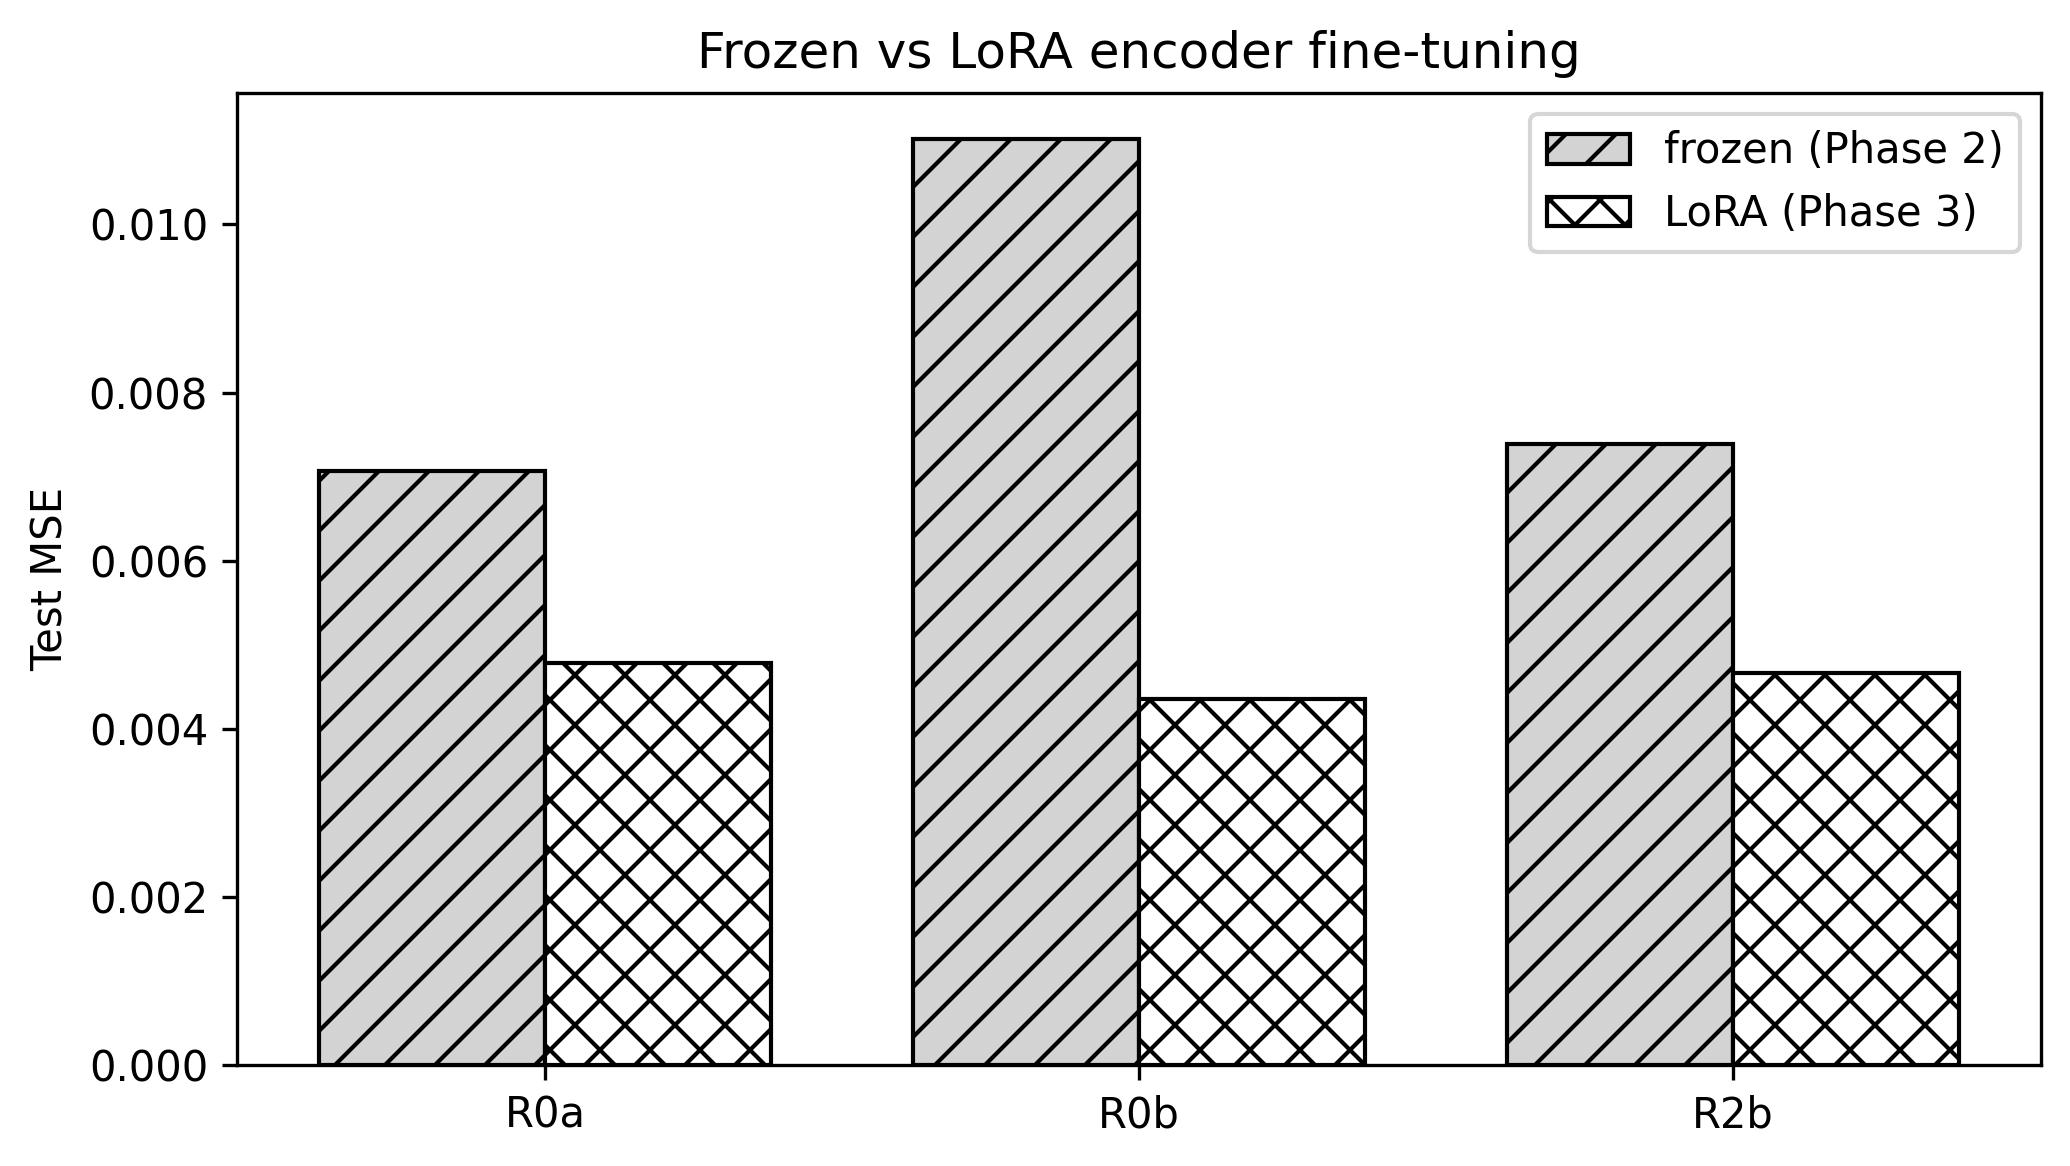
\includegraphics[width=\linewidth]{phase3_frozen_vs_lora.png}

\column{0.50\textwidth}
\small
\renewcommand{\arraystretch}{1.1}
\begin{tabular}{@{}lccc@{}}
\toprule
& \textbf{Frozen} & \textbf{LoRA} & \textbf{$\Delta$} \\
\midrule
R0a & 0.00707 & 0.00478 & \textcolor{ok}{$-$32\,\%} \\
R0b & 0.01101 & \textbf{0.00435} & \textcolor{ok}{$-$60\,\%} \\
R2b & 0.00739 & 0.00466 & \textcolor{ok}{$-$37\,\%} \\
\bottomrule
\end{tabular}
\medskip

\footnotesize
\begin{itemize}\setlength\itemsep{1pt}
  \item LoRA ($r{=}8$, $\alpha{=}16$, last 6 blocks)
  \item Only MLP projections adapted (attention MHA bypasses module forward)
  \item Gradient clipping (max-norm 1.0) fixed R0a divergence
  \item Online training, $\sim$84\,s/epoch on M4
\end{itemize}
\end{columns}
\end{frame}

% ---------- 9. REGIME REVERSAL + RLEAK ----------
\begin{frame}{Regime Reversal + Leakage Quantified}
\begin{columns}[T]
\column{0.50\textwidth}
\textbf{Regime reversal:}\\[4pt]
\small
\renewcommand{\arraystretch}{1.05}
\begin{tabular}{@{}lc@{}}
Frozen: & R0a (0.0071) $\ll$ R0b (0.0110) \\
        & \textcolor{accent}{cross-attn \textbf{helps}} \\[4pt]
LoRA:   & R0b (0.0044) $<$ R2b (0.0047) $<$ R0a (0.0048) \\
        & \textcolor{warn}{pure-vision \textbf{wins};} \\
        & fusion now redundant \\
\end{tabular}
\medskip

\footnotesize
Once the encoder can adapt, the fusion layer's capacity contribution
becomes unnecessary --- the visual pathway dominates.

\column{0.50\textwidth}
\centering
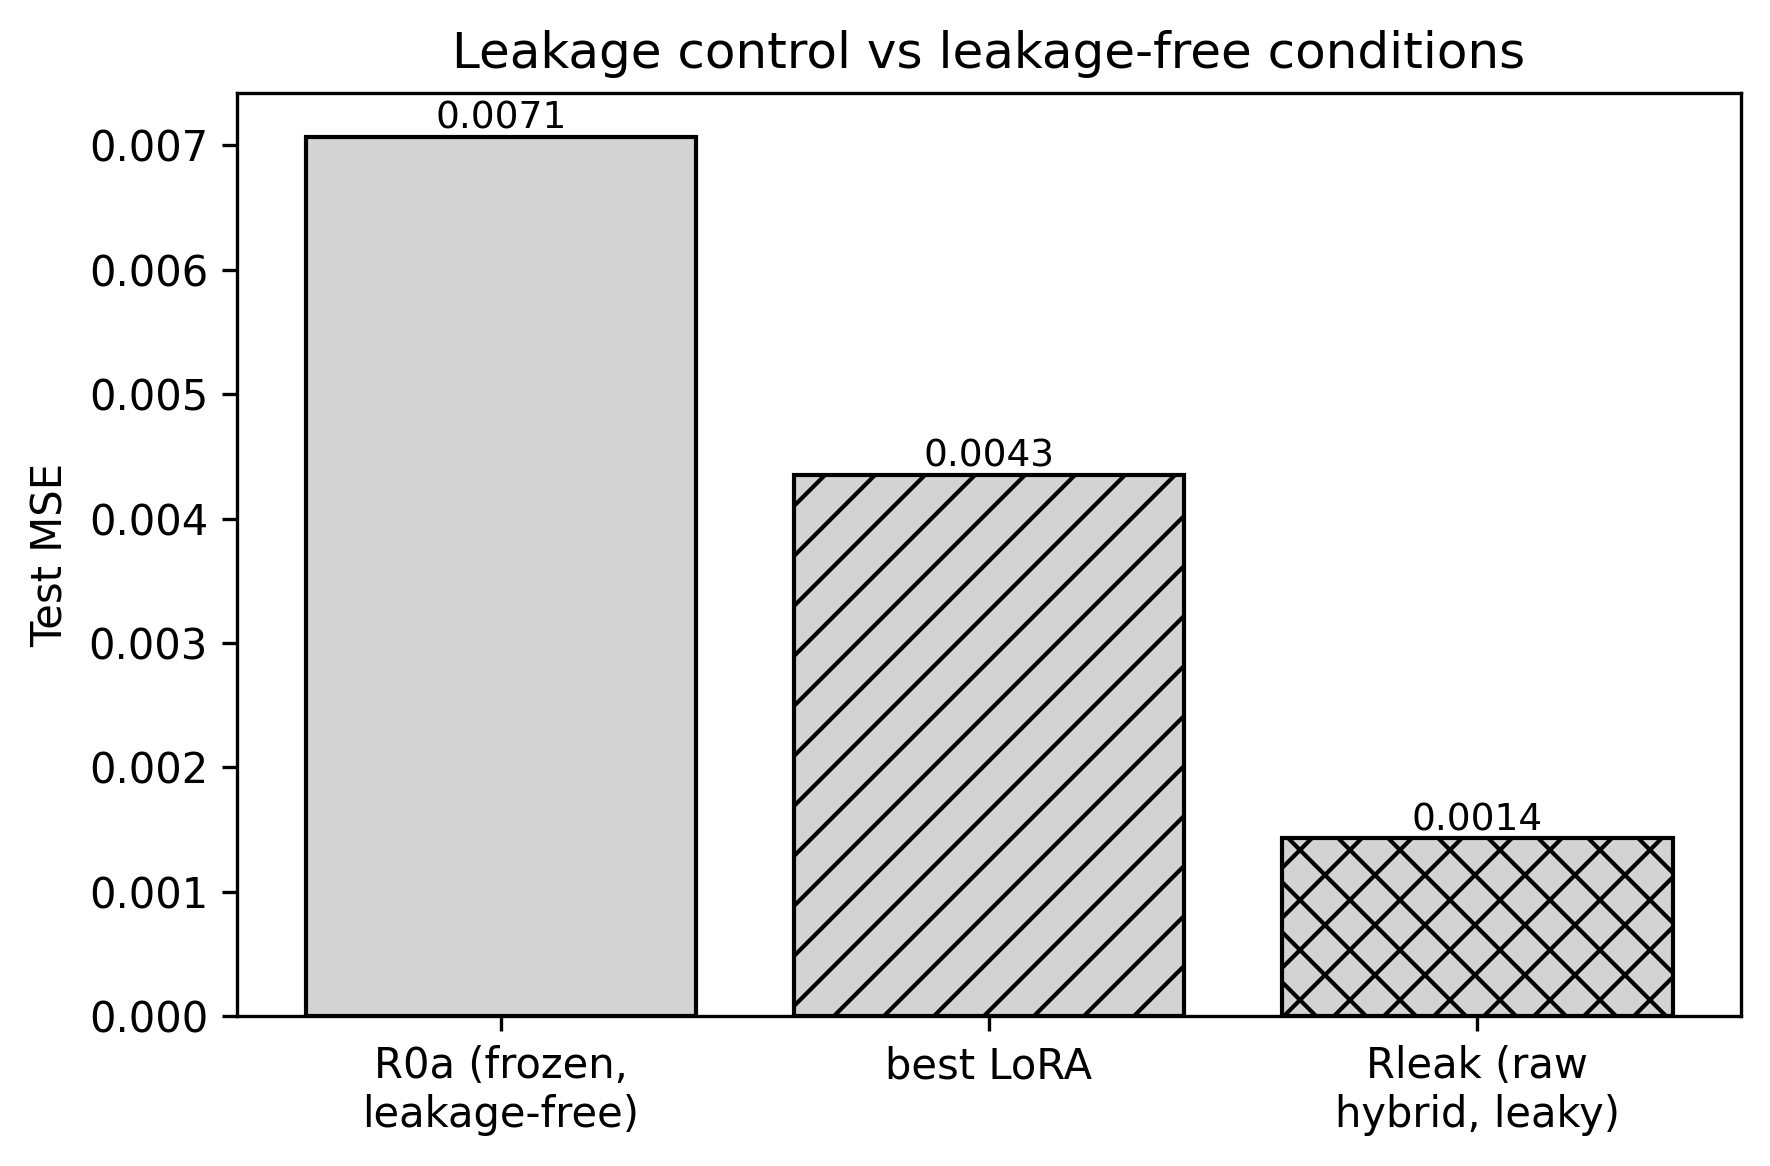
\includegraphics[width=0.92\linewidth]{phase3_leakage.png}\\[4pt]
\textbf{Rleak} (raw hybrid, GT \% intact) = \textbf{0.00143}\\
$\approx$ \textbf{1/3} of best leakage-free model\\
$\approx$ \textbf{1/5} of frozen R0a\\[4pt]
\footnotesize
\textcolor{warn}{The model copies the answer from text.}\\
Leakage failure mode \textbf{quantified}, not just asserted.
\end{columns}
\end{frame}

% ---------- 10. CODE BASE ----------
\begin{frame}[fragile]{Code Base \& Reproducibility}
\begin{columns}[T]
\column{0.55\textwidth}
\small
\begin{verbatim}
src/
├── dataset.py     7 conditions, 70/15/15
├── sanitize.py    regex + spaCy + fidelity
├── model.py       2 regressors + freeze flag
├── train.py       AdamW, cosine, W&B, LoRA
├── eval.py        metrics + attention viz
├── precompute.py  CLIP cache (image+text)
└── lora.py        LoRALinear + inject_lora

notebooks/
├── phase-1/phase1_poc.ipynb
├── phase-2/phase2_main.ipynb
└── phase-3/phase3_main.ipynb
\end{verbatim}

\column{0.45\textwidth}
\textbf{Reproducibility:}
\begin{itemize}\setlength\itemsep{2pt}\small
  \item \texttt{requirements.txt}
  \item Deterministic 70/15/15 (seed 42)
  \item 3 training seeds: 42, 1337, 2024
  \item Heavy artefacts gitignored
\end{itemize}
\medskip

\textbf{Tracking:}\\[2pt]
\small
\texttt{wandb.ai/mereyomerfaruk/}\\
\texttt{di725-project} --- 18 runs
\end{columns}
\end{frame}

% ---------- 11. LIVE DEMO ----------
\begin{frame}{Live Demo}
\centering
\Large \textbf{Switching to notebook \texttt{phase3\_main.ipynb}}
\medskip

\normalsize
Will show, in order:
\medskip

\begin{itemize}\setlength\itemsep{4pt}
  \item \textbf{\S2 Rleak training} --- per-epoch loss converging
  \item \textbf{\S4 evaluation table} --- mean $\pm$ std across seeds
  \item \textbf{\S5 frozen-vs-LoRA bar chart} --- live render
  \item \textbf{W\&B project page} --- 18 runs, validation curves
\end{itemize}

\vspace{1.5em}
\footnotesize
\textcolor{accent}{Per spec \S4.4.1: ``explain the code base, how to run it,
and demonstrate how it runs.''}
\end{frame}

% ---------- 12. CONCLUSIONS ----------
\begin{frame}{Conclusions}
\begin{enumerate}\setlength\itemsep{6pt}
\item \textbf{Fidelity, not richness, gates the effect.}\\
  {\small Clean captions help \emph{only} when they correctly describe the image;
   wins and losses cancel on average.}

\item \textbf{Architecture vs.\ content is regime-dependent.}\\
  {\small Frozen: cross-attention drives the gain.
   LoRA: pure-vision wins; fusion redundant.}

\item \textbf{Leakage quantified, not just asserted.}\\
  {\small Rleak $\approx$ 1/5 of frozen R0a --- the failure mode is real and measurable.}

\item \textbf{Methodological takeaway:}\\
  {\small multimodal gains must be ablated against
   architecture-matched no-text, random-text, \emph{and}
   fidelity-stratified baselines before any non-trivial text
   contribution is claimed.}
\end{enumerate}

\vfill
\centering
\large \textbf{Thank you.}\\[4pt]
{\footnotesize\href{https://github.com/OmerFarukMerey/remote-sensing-caption-composition}{github.com/OmerFarukMerey/remote-sensing-caption-composition}}\\
{\footnotesize\href{https://wandb.ai/mereyomerfaruk/di725-project}{wandb.ai/mereyomerfaruk/di725-project}}
\end{frame}

\end{document}
